\documentclass{article}

\usepackage{kotex}
\usepackage{fancyhdr}
\usepackage{extramarks}
\usepackage{amsmath}
\usepackage{amsthm}
\usepackage{amsfonts}
\usepackage{amssymb}
\usepackage{tikz}
\usepackage[plain]{algorithm}
\usepackage{algpseudocode}

\usetikzlibrary{automata,positioning}

%
% Basic Document Settings
%

\topmargin=-0.45in
\evensidemargin=0in
\oddsidemargin=0in
\textwidth=6.5in
\textheight=9.0in
\headsep=0.25in

\linespread{1.1}

\pagestyle{fancy}
\lhead{\hmwkAuthorName}
\chead{\hmwkClass\ (\hmwkClassInstructor): \hmwkTitle}
\rhead{\firstxmark}
\lfoot{\lastxmark}
\cfoot{\thepage}

\renewcommand\headrulewidth{0.4pt}
\renewcommand\footrulewidth{0.4pt}

\setlength\parindent{0pt}

\newcommand\numberthis{\addtocounter{equation}{1}\tag{\theequation}}

%
% Create Problem Sections
%

\newcommand{\enterProblemHeader}[1]{
    \nobreak\extramarks{}{Problem \arabic{#1} continued on next page\ldots}\nobreak{}
    \nobreak\extramarks{Problem \arabic{#1} (continued)}{Problem \arabic{#1} continued on next page\ldots}\nobreak{}
}

\newcommand{\exitProblemHeader}[1]{
    \nobreak\extramarks{Problem \arabic{#1} (continued)}{Problem \arabic{#1} continued on next page\ldots}\nobreak{}
    \stepcounter{#1}
    \nobreak\extramarks{Problem \arabic{#1}}{}\nobreak{}
}

\setcounter{secnumdepth}{0}
\newcounter{partCounter}
\newcounter{homeworkProblemCounter}
\setcounter{homeworkProblemCounter}{1}
\nobreak\extramarks{Problem \arabic{homeworkProblemCounter}}{}\nobreak{}

%
% Homework Problem Environment
%
% This environment takes an optional argument. When given, it will adjust the
% problem counter. This is useful for when the problems given for your
% assignment aren't sequential. See the last 3 problems of this template for an
% example.
%
\newenvironment{homeworkProblem}[1][-1]{
    \ifnum#1>0
        \setcounter{homeworkProblemCounter}{#1}
    \fi
    \section{Problem \arabic{homeworkProblemCounter}}
    \setcounter{partCounter}{1}
    \enterProblemHeader{homeworkProblemCounter}
}{
    \exitProblemHeader{homeworkProblemCounter}
}

%
% Homework Details
%   - Title
%   - Due date
%   - Class
%   - Section/Time
%   - Instructor
%   - Author
%

\newcommand{\hmwkTitle}{Homework\ \#6}
\newcommand{\hmwkDueDate}{December 13, 2016}
\newcommand{\hmwkClass}{CS300}
\newcommand{\hmwkClassInstructor}{Prof. Sunghee Choi}
\newcommand{\hmwkAuthorName}{Ohjun Kwon}

%
% Title Page
%

\title{
    \vspace{2in}
    \textmd{\textbf{\hmwkClass:\ \hmwkTitle}}\\
    \normalsize\vspace{0.1in}\small{Due\ on\ \hmwkDueDate\ at 10:30am}\\
    \vspace{0.1in}\large{\textit{\hmwkClassInstructor}}
    \vspace{3in}
}

\author{\textbf{20160051 \hmwkAuthorName}}
\date{}

\renewcommand{\part}{\textbf{\large Part \Alph{partCounter}}\stepcounter{partCounter}\\}

%
% Various Helper Commands
%

% Useful for algorithms
\newcommand{\alg}[1]{\textsc{\bfseries \footnotesize #1}}

% For derivatives
\newcommand{\deriv}[1]{\frac{\mathrm{d}}{\mathrm{d}x} (#1)}

% For partial derivatives
\newcommand{\pderiv}[2]{\frac{\partial}{\partial #1} (#2)}

% Integral dx
\newcommand{\dx}{\mathrm{d}x}

% Alias for the Solution section header
\newcommand{\solution}{\textbf{\large Solution}}

% Probability commands: Expectation, Variance, Covariance, Bias
\newcommand{\E}{\mathrm{E}}
\newcommand{\Var}{\mathrm{Var}}
\newcommand{\Cov}{\mathrm{Cov}}
\newcommand{\Bias}{\mathrm{Bias}}

\begin{document}

\maketitle

\pagebreak
\begin{homeworkProblem}
    문제에서 제시된 방향 비순환 그래프에서의 위상 정렬을 수행하는 방법의 단계를 크게 나누어보면,
    \begin{itemize}
        \item indegree가 0인 모든 정점을 찾는다.
        \item 위에서 찾은 정점과 그 정점에서 나가는 모든 간선을 삭제한다.
        \item 위에서 간선을 삭제함에 따라 연결된 정점의 indegree가 바뀌는 것을 반영하여
            만약 indegree가 0인 정점이 나오게 되면 그 정점을 위의 단계에 포함시킨다.
    \end{itemize}
    이렇게 크게 세 단계로 나누어 볼 수 있을 것이다.
    여기서 첫 번째 단계를 실행하기 위해서는 모든 정점에 대해서 간선을 탐색하며 indegree를 저장해야 하는데,
    인접그래프를 이용하여 그래프를 표현했다면 이를 계산하는데 드는 시간은 $O(V+E)$일 것이다.
    계산 후 indegree가 0인 모든 정점을 큐에 집어넣고 하나씩 pop하면서 그에 연결된 정점에 대해
    전에 계산된 indegree값을 1씩 빼면서 간선을 제거한다. 만약 이 과정에서 indegree의 값이 0이 되었다면
    그 정점을 큐에 넣어주면 된다. 이 과정을 모든 정점과 그 간선에 대해 시행되므로 $O(V+E)$의 시간이 소요될 것이다.
    그러므로 총 $O(V+E)$의 시간 복잡도가 된다.
    (Python 3으로 구현된 해당하는 알고리즘은 풀이의 맨 뒤에 첨부되어있다.)

    이러한 알고리즘이 성립되는 이유는 큐에 들어간 원소의 indegree가 0이기 때문이다.
    어떠한 정점이 큐에 들어갔다는 말은 indegree가 0이라는 소리이고, 이는 그에 도달하는 간선이 없다는 말이다.
    다시 말해, 그 정점에 도달하는 간선이 전에 큐에 들어갔다 나오면서 제거되었거나 처음부터 없었다는 이야기가 되는데,
    이는 바로 그에 대한 ``상위'' 정점이 이미 이전에 나왔다는 말이고, 위상 정렬이 되었다는 말과 같다.
    하지만 그래프에 순환이 있게 되면, 큐를 비우며 간선을 제거하는 도중 모든 정점이 자신의 ``상위'' 정점을
    갖게 되는 순간이 오게 된다. 다시 말해, indegree가 0인 정점이 없어진다. 왜냐하면, 순환에서는 간선이 순환하며
    연결이 되어 있기 때문에 모두 자신을 지목하는 정점을 가지게 되기 때문이다. 이 상황에서는 indegree가 0인 정점이
    더 이상 나오지 않기 때문에 모든 정점이 큐에 들어갔다 나오지는 않았지만 큐는 비게 되고, 순환에 포함된 정점을 남겨놓고
    알고리즘은 종료되게 된다.
\end{homeworkProblem}

\begin{homeworkProblem}
    \textbf{Proof}\\
    만약 거리가 $\delta (a,b)$인 $a$, $b$가 존재한다고 하자. ($\delta(a,b)\geq\delta(u,v)$) $X$를 root로 하여 tree를 그리면 그림~\ref{fig:2-1}처럼 그릴 수 있을 것이다.
    왜냐하면 일단 $u$와 $v$에는 자식 노드가 있게 되면 주어진 알고리즘 2, 3번째 줄의 가정과 맞지 않게 되므로 $u$, $v$는 단말 노드이고,
    트리에서는 어떠한 노드를 root로 잡아도 트리를 그릴 수 있으며, 두 노드 사이에는 반드시 하나의 경로만이 있기 때문이다.
    $r$과 $R$을 각각 $u$, $v$와 $a$, $b$에서 최초로 만나는 공통부모라고 하자. 여기서 $r$과 $R$은 서로 같을 수도 있고 다를 수도 있으며
    심지어는 $X$와도 같을 수 있다.
    \begin{figure}[!htb]
        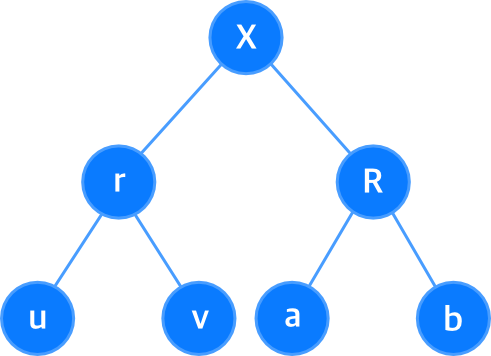
\includegraphics[height=0.2\textheight]{2-1}
        \centering
        \caption{트리}
        \label{fig:2-1}
    \end{figure}
    그림~\ref{fig:2-1}처럼 트리를 그리면 우리는 아래 두 부등식을 알 수 있다.
    \begin{align}
        \delta (X,r)+\delta (r,u)&\geq \delta(X,R)+\delta(R,a)\label{eq:2-1}\\
        \delta(r,v)&\geq\delta(r,R)+\delta(R,b)\label{eq:2-2}
    \end{align}
    식~\ref{eq:2-1}\은 $u$가 $X$에서 가장 멀리 떨어져 있다는 주어진 알고리즘의 두 번째 줄에 해당하는 가정이고,
    식~\ref{eq:2-2}\은 $v$가 $u$에서 가장 멀리 떨어져 있다는 주어진 알고리즘에 세 번쨰 줄에 해당하는 가정이다.
    이 두 부등식의 양변을 더하고 정리해주게 되면 아래 식~\ref{eq:2-3}\과 같은 식이 된다.
    \begin{align*}
        \delta(u,r)+\delta(r,v)+\delta(r,X)&\geq\delta(r,R)+\delta(X,R)+\delta(a,R)+\delta(R,b)\\
        \delta(u,v)&\geq(\delta(r,R)-\delta(r,X))+\delta(X,R)+\delta(a,b)\\
        \delta(u,v)&\geq2\delta(X,R)+\delta(a,b)\\
        &\geq\delta(a,b)\numberthis\label{eq:2-3}
    \end{align*}
    $\therefore \delta(u,v)\geq\delta(a,b)$이므로 $\delta(u,v)=\delta(a,b)$가 되어 결국 거리는 $\delta(u,v)$가 됨을 알 수 있다.
    \\

    \textbf{Analyze}\\
    주어진 알고리즘은 총 4줄로 이루어져 있는데 이를 한 줄씩 분석해보도록 하자.
    우선 첫 번째 줄은 주어진 그래프에서 임의의 정점 하나를 잡는 과정이므로 $O(1)$에 마칠 수 있다.
    두 번째 줄은 그래프에 대해 BFS를 수행하는 과정인데, 인접 리스트로 표현된 그래프에서 BFS는 $O(V+E)$에, 인접 행렬로 표현된 BFS는
    $O(V^2)$에 할 수 있다고 \textbf{Homework \#5}와 수업 시간에 보였으므로 계산은 생략한다.
    세 번째 줄도 두 번째 줄과 마찬가지로 BFS를 해주는 과정이므로 $O(V+E)$의 시간이 소요된다.
    네 번째 줄은 $u$에서 $v$까지의 최소 거리를 찾는 과정인데 음수의 가중치를 갖지 않으므로
    이는 다익스트라 알고리즘을 이용하면 구할 수 있고 시간 복잡도는 $O(E+V\lg V)$가 된다.
    그러므로 총 시간 복잡도는 $O(E+V\lg V)$가 된다.
\end{homeworkProblem}

\begin{homeworkProblem}
    \part
    주어진 결정 문제가 NP에 속하는지 확인하기 위해서는 다항 시간 안에 검증이 가능한지 확인해보아야 한다.
    주어진 경로 $(v_1, v_2, \dots, v_n)$이 해밀토니안 경로인지 다항 시간에 확인할 수 있는 알고리즘을 제시한다면
    주어진 결정 문제가 NP에 속한다고 증명할 수 있다.
    주어진 경로가 그래프 $G$의 $u$에서 $v$로의 해밀토니안 경로인지 확인하기 위해서는 다음 사실을 확인해보면 된다.
    \begin{itemize}
        \item $v_1=u$, $v_n=v$인가?
        \item 주어진 경로 내에 겹치는 정점은 없는가?
        \item 주어진 경로 내의 정점은 그래프 $G$에 존재하는 정점인가?
        \item 주어진 경로 내의 간선은 그래프 $G$에 존재하는 간선인가?
        \item 주어진 경로가 그래프 $G$의 모든 정점을 방문하는가?
    \end{itemize}
    첫 번째 사실은 직접 점들을 비교하면 되므로 $O(1)$만에 가능하고, 두 번째 사실은 주어진 경로 내에서 서로 다른 첨자 $i$, $j$에
    대해 전부 비교하면 되므로 $O(n^2)$에 가능하다. 세 번째 점은 주어진 경로 내의 각 점에 대하여 그래프 $G$의 정점의 집합 $V$에 속하는지
    확인하면 되므로 $O(nV)$에 가능하다. 네 번째 점은 첨자 $i\in[1,n-1]$에 대하여 간선 $(v_i,v_{i+1})$이 그래프
    $G$의 간선들의 집합 $E$에 속하는지 확인하면 되므로 $O(nE)$에 가능하다. (주어진 경로의 간선은 총 $n-1$개 이므로)
    마지막 사실은 위의 사실이 전부 확인된 상태에서 그래프 $G$의 정점의 집합 $V$의 원소의 개수와 집합 $\{v_1, \dots, v_n\}$의
    원소의 개수인 $n$이 같은지만 확인하면 되므로 $O(1)$에 확인할 수 있다. 그러므로 총 $O(V^2)$에 확인할 수 있으므로
    주어진 결정문제는 NP이다.
    \\

    \part
    방향 비순환 그래프에서 해밀토니안 경로가 있는지 확인하는 방법에는 우리가 1번에서 제시한 위상 정렬을 이용하면 된다.
    주어진 방향 비순환 그래프를 위상 정렬한 후, 각 정점이 차례로 다음 정점으로 연결되어 있는지 확인하면 된다.
    만약 연결이 되어 있다면 위상 정렬이 되어있는 순서가 바로 주어진 그래프의 해밀토니안 경로가 되고,
    그러한 연결이 존재하지 않는다면 주어진 그래프에서의 해밀토니안 경로는 존재하지 않는 것이 된다.
    이가 성립하는 이유는 위상 정렬이 된 상황에서 역으로 연결되는 간선이 존재하지 않기 때문이다.
    그러므로 차례대로 연결이 되어 있어야 한다.
    이 알고리즘의 시간 복잡도는 위상 정렬을 하는데 걸리는 시간과 차례로 연결되어 있는지 확인하는 시간의 합이 될 것인데,
    위상 정렬을 하는데에는 $O(V+E)$의 시간이 걸린다고 위에서 증명했고, 차례로 연결되어 있는지 확인하는데는 
    각 정점에 대해 각 간선을 한 번씩만 확인하면 되므로 $O(V+E)$의 시간이 걸린다.
    그러므로 주어진 결정 문제는 다항 시간 내로 풀 수 있다.
\end{homeworkProblem}
\end{document}
